\documentclass[1p]{elsarticle_modified}
%\bibliographystyle{elsarticle-num}

%\usepackage[colorlinks]{hyperref}
%\usepackage{abbrmath_seonhwa} %\Abb, \Ascr, \Acal ,\Abf, \Afrak
\usepackage{amsfonts}
\usepackage{amssymb}
\usepackage{amsmath}
\usepackage{amsthm}
\usepackage{scalefnt}
\usepackage{amsbsy}
\usepackage{kotex}
\usepackage{caption}
\usepackage{subfig}
\usepackage{color}
\usepackage{graphicx}
\usepackage{xcolor} %% white, black, red, green, blue, cyan, magenta, yellow
\usepackage{float}
\usepackage{setspace}
\usepackage{hyperref}

\usepackage{tikz}
\usetikzlibrary{arrows}

\usepackage{multirow}
\usepackage{array} % fixed length table
\usepackage{hhline}

%%%%%%%%%%%%%%%%%%%%%
\makeatletter
\renewcommand*\env@matrix[1][\arraystretch]{%
	\edef\arraystretch{#1}%
	\hskip -\arraycolsep
	\let\@ifnextchar\new@ifnextchar
	\array{*\c@MaxMatrixCols c}}
\makeatother %https://tex.stackexchange.com/questions/14071/how-can-i-increase-the-line-spacing-in-a-matrix
%%%%%%%%%%%%%%%

\usepackage[normalem]{ulem}

\newcommand{\msout}[1]{\ifmmode\text{\sout{\ensuremath{#1}}}\else\sout{#1}\fi}
%SOURCE: \msout is \stkout macro in https://tex.stackexchange.com/questions/20609/strikeout-in-math-mode

\newcommand{\cancel}[1]{
	\ifmmode
	{\color{red}\msout{#1}}
	\else
	{\color{red}\sout{#1}}
	\fi
}

\newcommand{\add}[1]{
	{\color{blue}\uwave{#1}}
}

\newcommand{\replace}[2]{
	\ifmmode
	{\color{red}\msout{#1}}{\color{blue}\uwave{#2}}
	\else
	{\color{red}\sout{#1}}{\color{blue}\uwave{#2}}
	\fi
}

\newcommand{\Sol}{\mathcal{S}} %segment
\newcommand{\D}{D} %diagram
\newcommand{\A}{\mathcal{A}} %arc


%%%%%%%%%%%%%%%%%%%%%%%%%%%%%5 test

\def\sl{\operatorname{\textup{SL}}(2,\Cbb)}
\def\psl{\operatorname{\textup{PSL}}(2,\Cbb)}
\def\quan{\mkern 1mu \triangleright \mkern 1mu}

\theoremstyle{definition}
\newtheorem{thm}{Theorem}[section]
\newtheorem{prop}[thm]{Proposition}
\newtheorem{lem}[thm]{Lemma}
\newtheorem{ques}[thm]{Question}
\newtheorem{cor}[thm]{Corollary}
\newtheorem{defn}[thm]{Definition}
\newtheorem{exam}[thm]{Example}
\newtheorem{rmk}[thm]{Remark}
\newtheorem{alg}[thm]{Algorithm}

\newcommand{\I}{\sqrt{-1}}
\begin{document}

%\begin{frontmatter}
%
%\title{Boundary parabolic representations of knots up to 8 crossings}
%
%%% Group authors per affiliation:
%\author{Yunhi Cho} 
%\address{Department of Mathematics, University of Seoul, Seoul, Korea}
%\ead{yhcho@uos.ac.kr}
%
%
%\author{Seonhwa Kim} %\fnref{s_kim}}
%\address{Center for Geometry and Physics, Institute for Basic Science, Pohang, 37673, Korea}
%\ead{ryeona17@ibs.re.kr}
%
%\author{Hyuk Kim}
%\address{Department of Mathematical Sciences, Seoul National University, Seoul 08826, Korea}
%\ead{hyukkim@snu.ac.kr}
%
%\author{Seokbeom Yoon}
%\address{Department of Mathematical Sciences, Seoul National University, Seoul, 08826,  Korea}
%\ead{sbyoon15@snu.ac.kr}
%
%\begin{abstract}
%We find all boundary parabolic representation of knots up to 8 crossings.
%
%\end{abstract}
%\begin{keyword}
%    \MSC[2010] 57M25 
%\end{keyword}
%
%\end{frontmatter}

%\linenumbers
%\tableofcontents
%
\newcommand\colored[1]{\textcolor{white}{\rule[-0.35ex]{0.8em}{1.4ex}}\kern-0.8em\color{red} #1}%
%\newcommand\colored[1]{\textcolor{white}{ #1}\kern-2.17ex	\textcolor{white}{ #1}\kern-1.81ex	\textcolor{white}{ #1}\kern-2.15ex\color{red}#1	}

{\Large $\underline{11n_{182}~(K11n_{182})}$}

\setlength{\tabcolsep}{10pt}
\renewcommand{\arraystretch}{1.6}
\vspace{1cm}\begin{tabular}{m{100pt}>{\centering\arraybackslash}m{274pt}}
\multirow{5}{120pt}{
	\centering
	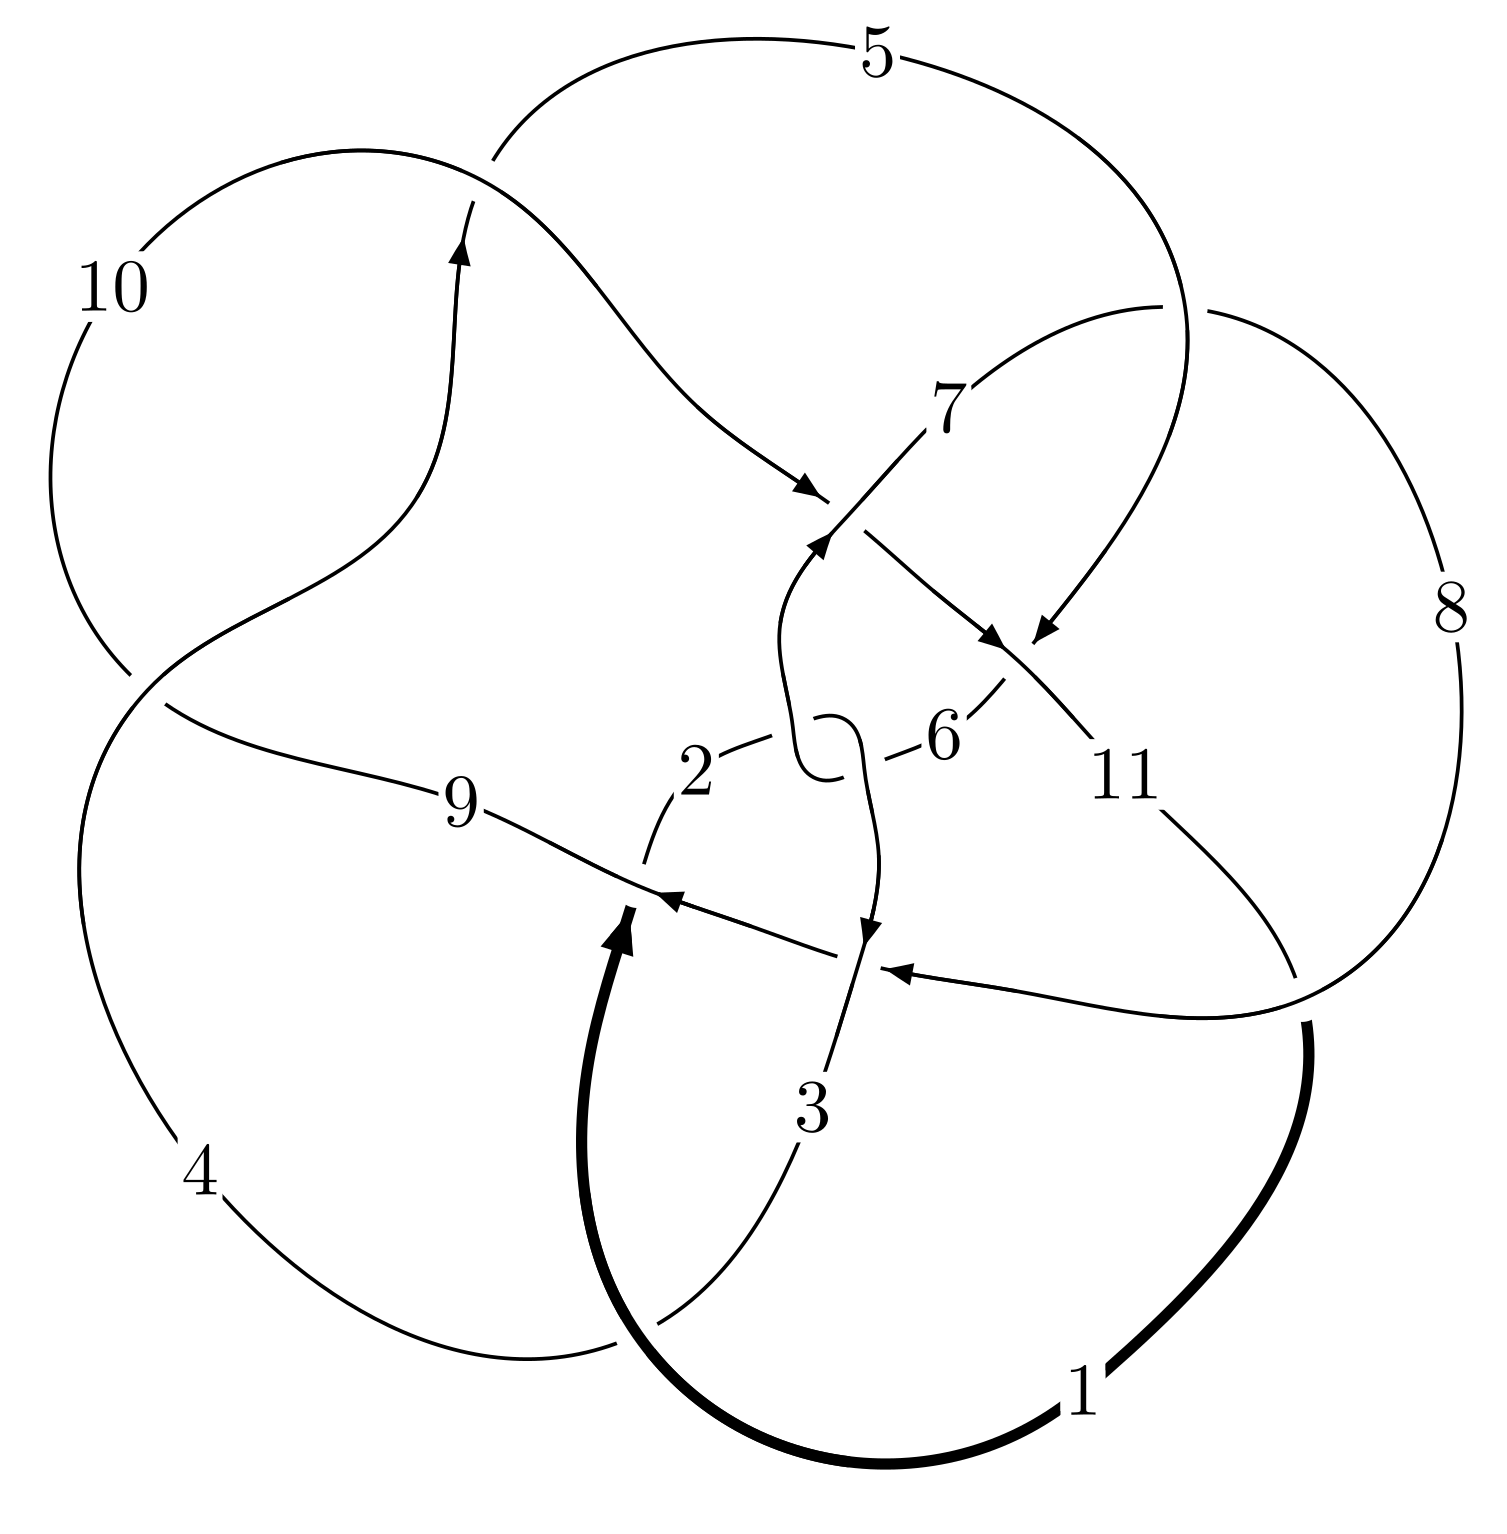
\includegraphics[width=112pt]{../../../GIT/diagram.site/Diagrams/png/798_11n_182.png}\\
\ \ \ A knot diagram\footnotemark}&
\allowdisplaybreaks
\textbf{Linearized knot diagam} \\
\cline{2-2}
 &
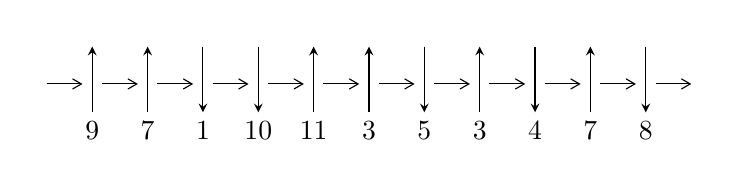
\begin{tikzpicture}[x=20pt, y=17pt]
	% nodes
	\node (C0) at (0, 0) {};
	\node (C1) at (1, 0) {};
	\node (C1U) at (1, +1) {};
	\node (C1D) at (1, -1) {9};

	\node (C2) at (2, 0) {};
	\node (C2U) at (2, +1) {};
	\node (C2D) at (2, -1) {7};

	\node (C3) at (3, 0) {};
	\node (C3U) at (3, +1) {};
	\node (C3D) at (3, -1) {1};

	\node (C4) at (4, 0) {};
	\node (C4U) at (4, +1) {};
	\node (C4D) at (4, -1) {10};

	\node (C5) at (5, 0) {};
	\node (C5U) at (5, +1) {};
	\node (C5D) at (5, -1) {11};

	\node (C6) at (6, 0) {};
	\node (C6U) at (6, +1) {};
	\node (C6D) at (6, -1) {3};

	\node (C7) at (7, 0) {};
	\node (C7U) at (7, +1) {};
	\node (C7D) at (7, -1) {5};

	\node (C8) at (8, 0) {};
	\node (C8U) at (8, +1) {};
	\node (C8D) at (8, -1) {3};

	\node (C9) at (9, 0) {};
	\node (C9U) at (9, +1) {};
	\node (C9D) at (9, -1) {4};

	\node (C10) at (10, 0) {};
	\node (C10U) at (10, +1) {};
	\node (C10D) at (10, -1) {7};

	\node (C11) at (11, 0) {};
	\node (C11U) at (11, +1) {};
	\node (C11D) at (11, -1) {8};
	\node (C12) at (12, 0) {};

	% arrows
	\draw[->,>={angle 60}]
	(C0) edge (C1) (C1) edge (C2) (C2) edge (C3) (C3) edge (C4) (C4) edge (C5) (C5) edge (C6) (C6) edge (C7) (C7) edge (C8) (C8) edge (C9) (C9) edge (C10) (C10) edge (C11) (C11) edge (C12) ;	\draw[->,>=stealth]
	(C1D) edge (C1U) (C2D) edge (C2U) (C3U) edge (C3D) (C4U) edge (C4D) (C5D) edge (C5U) (C6D) edge (C6U) (C7U) edge (C7D) (C8D) edge (C8U) (C9U) edge (C9D) (C10D) edge (C10U) (C11U) edge (C11D) ;
	\end{tikzpicture} \\
\hhline{~~} \\& 
\textbf{Solving Sequence} \\ \cline{2-2} 
 &
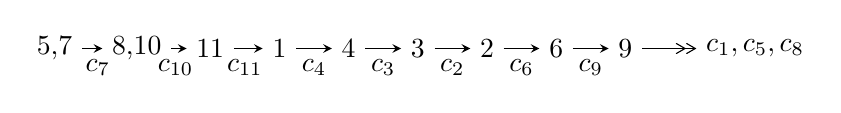
\begin{tikzpicture}[x=25pt, y=7pt]
	% node
	\node (A0) at (-1/8, 0) {5,7};
	\node (A1) at (17/16, 0) {8,10};
	\node (A2) at (17/8, 0) {11};
	\node (A3) at (25/8, 0) {1};
	\node (A4) at (33/8, 0) {4};
	\node (A5) at (41/8, 0) {3};
	\node (A6) at (49/8, 0) {2};
	\node (A7) at (57/8, 0) {6};
	\node (A8) at (65/8, 0) {9};
	\node (C1) at (1/2, -1) {$c_{7}$};
	\node (C2) at (13/8, -1) {$c_{10}$};
	\node (C3) at (21/8, -1) {$c_{11}$};
	\node (C4) at (29/8, -1) {$c_{4}$};
	\node (C5) at (37/8, -1) {$c_{3}$};
	\node (C6) at (45/8, -1) {$c_{2}$};
	\node (C7) at (53/8, -1) {$c_{6}$};
	\node (C8) at (61/8, -1) {$c_{9}$};
	\node (A9) at (10, 0) {$c_{1},c_{5},c_{8}$};

	% edge
	\draw[->,>=stealth]	
	(A0) edge (A1) (A1) edge (A2) (A2) edge (A3) (A3) edge (A4) (A4) edge (A5) (A5) edge (A6) (A6) edge (A7) (A7) edge (A8) ;
	\draw[->>,>={angle 60}]	
	(A8) edge (A9);
\end{tikzpicture} \\ 

\end{tabular} \\

\footnotetext{
The image of knot diagram is generated by the software ``\textbf{Draw programme}" developed by Andrew Bartholomew(\url{http://www.layer8.co.uk/maths/draw/index.htm\#Running-draw}), where we modified some parts for our purpose(\url{https://github.com/CATsTAILs/LinksPainter}).
}\phantom \\ \newline 
\centering \textbf{Ideals for irreducible components\footnotemark of $X_{\text{par}}$} 
 
\begin{align*}
I^u_{1}&=\langle 
-20148888016 u^{22}-749797203535 u^{21}+\cdots+2663810305417 b-383665719756,\\
\phantom{I^u_{1}}&\phantom{= \langle  }-10534409632231 u^{22}+12986341631640 u^{21}+\cdots+2663810305417 a-72898377806205,\\
\phantom{I^u_{1}}&\phantom{= \langle  }u^{23}- u^{22}+\cdots+5 u+1\rangle \\
I^u_{2}&=\langle 
-4.69374\times10^{59} u^{39}+1.06924\times10^{60} u^{38}+\cdots+3.76856\times10^{59} b+1.45903\times10^{61},\\
\phantom{I^u_{2}}&\phantom{= \langle  }6.35380\times10^{61} u^{39}-1.40886\times10^{62} u^{38}+\cdots+5.46442\times10^{61} a-2.06339\times10^{63},\;u^{40}-3 u^{39}+\cdots-25 u+29\rangle \\
I^u_{3}&=\langle 
-45306 u^{13}-181273 u^{12}+\cdots+142097 b+321146,\\
\phantom{I^u_{3}}&\phantom{= \langle  }803669 u^{13}+4740916 u^{12}+\cdots+142097 a+1220228,\\
\phantom{I^u_{3}}&\phantom{= \langle  }u^{14}+6 u^{13}+12 u^{12}+6 u^{11}-3 u^{10}+23 u^9+59 u^8+22 u^7-43 u^6-45 u^5-7 u^4+16 u^3+14 u^2+5 u+1\rangle \\
I^u_{4}&=\langle 
b+u+1,\;a,\;u^3+u^2-1\rangle \\
\\
\end{align*}
\raggedright * 4 irreducible components of $\dim_{\mathbb{C}}=0$, with total 80 representations.\\
\footnotetext{All coefficients of polynomials are rational numbers. But the coefficients are sometimes approximated in decimal forms when there is not enough margin.}
\newpage
\renewcommand{\arraystretch}{1}
\centering \section*{I. $I^u_{1}= \langle -2.01\times10^{10} u^{22}-7.50\times10^{11} u^{21}+\cdots+2.66\times10^{12} b-3.84\times10^{11},\;-1.05\times10^{13} u^{22}+1.30\times10^{13} u^{21}+\cdots+2.66\times10^{12} a-7.29\times10^{13},\;u^{23}- u^{22}+\cdots+5 u+1 \rangle$}
\flushleft \textbf{(i) Arc colorings}\\
\begin{tabular}{m{7pt} m{180pt} m{7pt} m{180pt} }
\flushright $a_{5}=$&$\begin{pmatrix}0\\u\end{pmatrix}$ \\
\flushright $a_{7}=$&$\begin{pmatrix}1\\0\end{pmatrix}$ \\
\flushright $a_{8}=$&$\begin{pmatrix}1\\u^2\end{pmatrix}$ \\
\flushright $a_{10}=$&$\begin{pmatrix}3.95464 u^{22}-4.87510 u^{21}+\cdots-45.3209 u+27.3662\\0.00756394 u^{22}+0.281475 u^{21}+\cdots+1.99017 u+0.144029\end{pmatrix}$ \\
\flushright $a_{11}=$&$\begin{pmatrix}3.96220 u^{22}-4.59362 u^{21}+\cdots-43.3307 u+27.5102\\0.00756394 u^{22}+0.281475 u^{21}+\cdots+1.99017 u+0.144029\end{pmatrix}$ \\
\flushright $a_{1}=$&$\begin{pmatrix}4.19771 u^{22}-4.99533 u^{21}+\cdots-46.1260 u+27.9976\\-0.296345 u^{22}+0.358714 u^{21}+\cdots+2.58565 u+0.310226\end{pmatrix}$ \\
\flushright $a_{4}=$&$\begin{pmatrix}-22.8331 u^{22}+26.1180 u^{21}+\cdots+253.774 u-151.915\\0.0861032 u^{22}-0.0646937 u^{21}+\cdots-0.600147 u+0.912866\end{pmatrix}$ \\
\flushright $a_{3}=$&$\begin{pmatrix}-22.0355 u^{22}+25.3812 u^{21}+\cdots+246.765 u-147.718\\0.0237345 u^{22}-0.319401 u^{21}+\cdots-2.39210 u+0.616521\end{pmatrix}$ \\
\flushright $a_{2}=$&$\begin{pmatrix}-22.0593 u^{22}+25.7006 u^{21}+\cdots+249.157 u-148.334\\0.0237345 u^{22}-0.319401 u^{21}+\cdots-2.39210 u+0.616521\end{pmatrix}$ \\
\flushright $a_{6}=$&$\begin{pmatrix}-22.6866 u^{22}+26.0341 u^{21}+\cdots+251.311 u-149.997\\0.0604215 u^{22}-0.0191991 u^{21}+\cdots+0.136923 u+1.00555\end{pmatrix}$ \\
\flushright $a_{9}=$&$\begin{pmatrix}-122.419 u^{22}+140.753 u^{21}+\cdots+1356.31 u-817.081\\0.550132 u^{22}-0.666197 u^{21}+\cdots-5.81233 u+4.35302\end{pmatrix}$\\ \flushright $a_{9}=$&$\begin{pmatrix}-122.419 u^{22}+140.753 u^{21}+\cdots+1356.31 u-817.081\\0.550132 u^{22}-0.666197 u^{21}+\cdots-5.81233 u+4.35302\end{pmatrix}$\\&\end{tabular}
\flushleft \textbf{(ii) Obstruction class $= -1$}\\~\\
\flushleft \textbf{(iii) Cusp Shapes $= \frac{94310497538971}{2663810305417} u^{22}-\frac{105799611203026}{2663810305417} u^{21}+\cdots-\frac{1045853706856708}{2663810305417} u+\frac{633409804939426}{2663810305417}$}\\~\\
\newpage\renewcommand{\arraystretch}{1}
\flushleft \textbf{(iv) u-Polynomials at the component}\newline \\
\begin{tabular}{m{50pt}|m{274pt}}
Crossings & \hspace{64pt}u-Polynomials at each crossing \\
\hline $$\begin{aligned}c_{1},c_{10}\end{aligned}$$&$\begin{aligned}
&u^{23}-6 u^{21}+\cdots-40 u-4
\end{aligned}$\\
\hline $$\begin{aligned}c_{2},c_{6}\end{aligned}$$&$\begin{aligned}
&u^{23}-3 u^{22}+\cdots+47 u-8
\end{aligned}$\\
\hline $$\begin{aligned}c_{3},c_{7}\end{aligned}$$&$\begin{aligned}
&u^{23}- u^{22}+\cdots+5 u+1
\end{aligned}$\\
\hline $$\begin{aligned}c_{4},c_{9}\end{aligned}$$&$\begin{aligned}
&u^{23}-9 u^{22}+\cdots-40 u+16
\end{aligned}$\\
\hline $$\begin{aligned}c_{5},c_{8}\end{aligned}$$&$\begin{aligned}
&u^{23}-6 u^{22}+\cdots+22 u-5
\end{aligned}$\\
\hline $$\begin{aligned}c_{11}\end{aligned}$$&$\begin{aligned}
&u^{23}+4 u^{22}+\cdots-7 u-34
\end{aligned}$\\
\hline
\end{tabular}\\~\\
\newpage\renewcommand{\arraystretch}{1}
\flushleft \textbf{(v) Riley Polynomials at the component}\newline \\
\begin{tabular}{m{50pt}|m{274pt}}
Crossings & \hspace{64pt}Riley Polynomials at each crossing \\
\hline $$\begin{aligned}c_{1},c_{10}\end{aligned}$$&$\begin{aligned}
&y^{23}-12 y^{22}+\cdots+448 y-16
\end{aligned}$\\
\hline $$\begin{aligned}c_{2},c_{6}\end{aligned}$$&$\begin{aligned}
&y^{23}-13 y^{22}+\cdots+1233 y-64
\end{aligned}$\\
\hline $$\begin{aligned}c_{3},c_{7}\end{aligned}$$&$\begin{aligned}
&y^{23}-5 y^{22}+\cdots+41 y-1
\end{aligned}$\\
\hline $$\begin{aligned}c_{4},c_{9}\end{aligned}$$&$\begin{aligned}
&y^{23}-43 y^{22}+\cdots-1088 y-256
\end{aligned}$\\
\hline $$\begin{aligned}c_{5},c_{8}\end{aligned}$$&$\begin{aligned}
&y^{23}-46 y^{22}+\cdots+344 y-25
\end{aligned}$\\
\hline $$\begin{aligned}c_{11}\end{aligned}$$&$\begin{aligned}
&y^{23}+6 y^{22}+\cdots-12055 y-1156
\end{aligned}$\\
\hline
\end{tabular}\\~\\
\newpage\flushleft \textbf{(vi) Complex Volumes and Cusp Shapes}
$$\begin{array}{c|c|c}  
\text{Solutions to }I^u_{1}& \I (\text{vol} + \sqrt{-1}CS) & \text{Cusp shape}\\
 \hline 
\begin{aligned}
u &= \phantom{-}0.555624 + 0.905584 I \\
a &= \phantom{-}0.910105 - 0.864749 I \\
b &= -1.40913 + 1.48491 I\end{aligned}
 & \phantom{-}1.86354 - 5.26744 I & \phantom{-}5.28915 + 6.74191 I \\ \hline\begin{aligned}
u &= \phantom{-}0.555624 - 0.905584 I \\
a &= \phantom{-}0.910105 + 0.864749 I \\
b &= -1.40913 - 1.48491 I\end{aligned}
 & \phantom{-}1.86354 + 5.26744 I & \phantom{-}5.28915 - 6.74191 I \\ \hline\begin{aligned}
u &= \phantom{-}1.08075\phantom{ +0.000000I} \\
a &= -0.674705\phantom{ +0.000000I} \\
b &= \phantom{-}2.01594\phantom{ +0.000000I}\end{aligned}
 & \phantom{-}5.56139\phantom{ +0.000000I} & -4.10580\phantom{ +0.000000I} \\ \hline\begin{aligned}
u &= \phantom{-}0.501300 + 0.715167 I \\
a &= -0.703633 - 0.411741 I \\
b &= \phantom{-}1.46848 - 0.46020 I\end{aligned}
 & \phantom{-}6.01384 - 1.36939 I & \phantom{-}7.91646 + 4.62007 I \\ \hline\begin{aligned}
u &= \phantom{-}0.501300 - 0.715167 I \\
a &= -0.703633 + 0.411741 I \\
b &= \phantom{-}1.46848 + 0.46020 I\end{aligned}
 & \phantom{-}6.01384 + 1.36939 I & \phantom{-}7.91646 - 4.62007 I \\ \hline\begin{aligned}
u &= \phantom{-}0.728418 + 0.872189 I \\
a &= -0.297023 + 0.916259 I \\
b &= -0.631160 - 0.422833 I\end{aligned}
 & \phantom{-}3.37848 + 2.40469 I & \phantom{-}1.77991 - 2.36658 I \\ \hline\begin{aligned}
u &= \phantom{-}0.728418 - 0.872189 I \\
a &= -0.297023 - 0.916259 I \\
b &= -0.631160 + 0.422833 I\end{aligned}
 & \phantom{-}3.37848 - 2.40469 I & \phantom{-}1.77991 + 2.36658 I \\ \hline\begin{aligned}
u &= -1.049550 + 0.569449 I \\
a &= \phantom{-}0.978794 + 0.476256 I \\
b &= -0.827795 - 0.239786 I\end{aligned}
 & -5.59031 + 2.93906 I & -3.96701 - 3.47635 I \\ \hline\begin{aligned}
u &= -1.049550 - 0.569449 I \\
a &= \phantom{-}0.978794 - 0.476256 I \\
b &= -0.827795 + 0.239786 I\end{aligned}
 & -5.59031 - 2.93906 I & -3.96701 + 3.47635 I \\ \hline\begin{aligned}
u &= -0.704512 + 0.984779 I \\
a &= \phantom{-}0.736671 + 0.559489 I \\
b &= -0.414106 - 1.231940 I\end{aligned}
 & -2.32908 + 5.49763 I & -4.79992 - 7.26042 I\\
 \hline 
 \end{array}$$\newpage$$\begin{array}{c|c|c}  
\text{Solutions to }I^u_{1}& \I (\text{vol} + \sqrt{-1}CS) & \text{Cusp shape}\\
 \hline 
\begin{aligned}
u &= -0.704512 - 0.984779 I \\
a &= \phantom{-}0.736671 - 0.559489 I \\
b &= -0.414106 + 1.231940 I\end{aligned}
 & -2.32908 - 5.49763 I & -4.79992 + 7.26042 I \\ \hline\begin{aligned}
u &= \phantom{-}0.929406 + 0.853194 I \\
a &= \phantom{-}0.740478 + 0.793412 I \\
b &= -1.091640 + 0.630699 I\end{aligned}
 & \phantom{-}5.11296 - 9.53315 I & \phantom{-}2.57549 + 7.49079 I \\ \hline\begin{aligned}
u &= \phantom{-}0.929406 - 0.853194 I \\
a &= \phantom{-}0.740478 - 0.793412 I \\
b &= -1.091640 - 0.630699 I\end{aligned}
 & \phantom{-}5.11296 + 9.53315 I & \phantom{-}2.57549 - 7.49079 I \\ \hline\begin{aligned}
u &= \phantom{-}0.734602\phantom{ +0.000000I} \\
a &= \phantom{-}1.84769\phantom{ +0.000000I} \\
b &= -0.838790\phantom{ +0.000000I}\end{aligned}
 & -3.46093\phantom{ +0.000000I} & \phantom{-}0.434270\phantom{ +0.000000I} \\ \hline\begin{aligned}
u &= -1.000300 + 0.806208 I \\
a &= \phantom{-}0.146523 - 0.473900 I \\
b &= -0.602615 - 0.205653 I\end{aligned}
 & -0.46558 + 3.81570 I & \phantom{-}4.70967 - 3.05268 I \\ \hline\begin{aligned}
u &= -1.000300 - 0.806208 I \\
a &= \phantom{-}0.146523 + 0.473900 I \\
b &= -0.602615 + 0.205653 I\end{aligned}
 & -0.46558 - 3.81570 I & \phantom{-}4.70967 + 3.05268 I \\ \hline\begin{aligned}
u &= -0.188306 + 0.473727 I \\
a &= -1.261830 + 0.253849 I \\
b &= \phantom{-}0.271244 + 0.415630 I\end{aligned}
 & \phantom{-}0.294559 + 1.131280 I & \phantom{-}2.80927 - 6.63257 I \\ \hline\begin{aligned}
u &= -0.188306 - 0.473727 I \\
a &= -1.261830 - 0.253849 I \\
b &= \phantom{-}0.271244 - 0.415630 I\end{aligned}
 & \phantom{-}0.294559 - 1.131280 I & \phantom{-}2.80927 + 6.63257 I \\ \hline\begin{aligned}
u &= -1.33922 + 0.68743 I \\
a &= -0.831149 - 0.099202 I \\
b &= \phantom{-}1.41488 + 0.83581 I\end{aligned}
 & -3.36043 + 7.89416 I & -1.16388 - 6.61187 I \\ \hline\begin{aligned}
u &= -1.33922 - 0.68743 I \\
a &= -0.831149 + 0.099202 I \\
b &= \phantom{-}1.41488 - 0.83581 I\end{aligned}
 & -3.36043 - 7.89416 I & -1.16388 + 6.61187 I\\
 \hline 
 \end{array}$$\newpage$$\begin{array}{c|c|c}  
\text{Solutions to }I^u_{1}& \I (\text{vol} + \sqrt{-1}CS) & \text{Cusp shape}\\
 \hline 
\begin{aligned}
u &= \phantom{-}1.23451 + 0.89988 I \\
a &= -0.999661 + 0.218042 I \\
b &= \phantom{-}1.34140 - 1.32358 I\end{aligned}
 & \phantom{-}0.6169 - 16.3897 I & -0.60357 + 8.49133 I \\ \hline\begin{aligned}
u &= \phantom{-}1.23451 - 0.89988 I \\
a &= -0.999661 - 0.218042 I \\
b &= \phantom{-}1.34140 + 1.32358 I\end{aligned}
 & \phantom{-}0.6169 + 16.3897 I & -0.60357 - 8.49133 I \\ \hline\begin{aligned}
u &= -0.150085\phantom{ +0.000000I} \\
a &= \phantom{-}36.9885\phantom{ +0.000000I} \\
b &= -0.216243\phantom{ +0.000000I}\end{aligned}
 & -0.0107219\phantom{ +0.000000I} & \phantom{-}320.580\phantom{ +0.000000I}\\
 \hline 
 \end{array}$$\newpage\newpage\renewcommand{\arraystretch}{1}
\centering \section*{II. $I^u_{2}= \langle -4.69\times10^{59} u^{39}+1.07\times10^{60} u^{38}+\cdots+3.77\times10^{59} b+1.46\times10^{61},\;6.35\times10^{61} u^{39}-1.41\times10^{62} u^{38}+\cdots+5.46\times10^{61} a-2.06\times10^{63},\;u^{40}-3 u^{39}+\cdots-25 u+29 \rangle$}
\flushleft \textbf{(i) Arc colorings}\\
\begin{tabular}{m{7pt} m{180pt} m{7pt} m{180pt} }
\flushright $a_{5}=$&$\begin{pmatrix}0\\u\end{pmatrix}$ \\
\flushright $a_{7}=$&$\begin{pmatrix}1\\0\end{pmatrix}$ \\
\flushright $a_{8}=$&$\begin{pmatrix}1\\u^2\end{pmatrix}$ \\
\flushright $a_{10}=$&$\begin{pmatrix}-1.16276 u^{39}+2.57824 u^{38}+\cdots+15.4232 u+37.7606\\1.24550 u^{39}-2.83726 u^{38}+\cdots-21.4581 u-38.7159\end{pmatrix}$ \\
\flushright $a_{11}=$&$\begin{pmatrix}0.0827388 u^{39}-0.259017 u^{38}+\cdots-6.03488 u-0.955344\\1.24550 u^{39}-2.83726 u^{38}+\cdots-21.4581 u-38.7159\end{pmatrix}$ \\
\flushright $a_{1}=$&$\begin{pmatrix}-1.18195 u^{39}+2.57423 u^{38}+\cdots+12.7538 u+38.0738\\0.434159 u^{39}-1.02128 u^{38}+\cdots-8.80280 u-10.8518\end{pmatrix}$ \\
\flushright $a_{4}=$&$\begin{pmatrix}0.296393 u^{39}-0.547600 u^{38}+\cdots+8.50789 u-11.9654\\0.237025 u^{39}-0.603121 u^{38}+\cdots-13.2225 u-4.41074\end{pmatrix}$ \\
\flushright $a_{3}=$&$\begin{pmatrix}-1.03486 u^{39}+2.43611 u^{38}+\cdots+28.2109 u+46.3778\\0.440164 u^{39}-0.996927 u^{38}+\cdots-8.56472 u-15.8344\end{pmatrix}$ \\
\flushright $a_{2}=$&$\begin{pmatrix}-1.47503 u^{39}+3.43303 u^{38}+\cdots+36.7756 u+62.2122\\0.440164 u^{39}-0.996927 u^{38}+\cdots-8.56472 u-15.8344\end{pmatrix}$ \\
\flushright $a_{6}=$&$\begin{pmatrix}0.246893 u^{39}-0.444760 u^{38}+\cdots+0.0495641 u-2.02219\\-0.286524 u^{39}+0.705961 u^{38}+\cdots+6.76415 u+14.3540\end{pmatrix}$ \\
\flushright $a_{9}=$&$\begin{pmatrix}1.94454 u^{39}-4.32792 u^{38}+\cdots-27.3144 u-65.7640\\-0.600066 u^{39}+1.33935 u^{38}+\cdots+6.52606 u+22.9357\end{pmatrix}$\\ \flushright $a_{9}=$&$\begin{pmatrix}1.94454 u^{39}-4.32792 u^{38}+\cdots-27.3144 u-65.7640\\-0.600066 u^{39}+1.33935 u^{38}+\cdots+6.52606 u+22.9357\end{pmatrix}$\\&\end{tabular}
\flushleft \textbf{(ii) Obstruction class $= -1$}\\~\\
\flushleft \textbf{(iii) Cusp Shapes $= 2.41432 u^{39}-4.79564 u^{38}+\cdots+14.4984 u-64.7958$}\\~\\
\newpage\renewcommand{\arraystretch}{1}
\flushleft \textbf{(iv) u-Polynomials at the component}\newline \\
\begin{tabular}{m{50pt}|m{274pt}}
Crossings & \hspace{64pt}u-Polynomials at each crossing \\
\hline $$\begin{aligned}c_{1},c_{10}\end{aligned}$$&$\begin{aligned}
&u^{40}+9 u^{38}+\cdots+244 u-44
\end{aligned}$\\
\hline $$\begin{aligned}c_{2},c_{6}\end{aligned}$$&$\begin{aligned}
&(u^{20}+2 u^{19}+\cdots+8 u+1)^{2}
\end{aligned}$\\
\hline $$\begin{aligned}c_{3},c_{7}\end{aligned}$$&$\begin{aligned}
&u^{40}-3 u^{39}+\cdots-25 u+29
\end{aligned}$\\
\hline $$\begin{aligned}c_{4},c_{9}\end{aligned}$$&$\begin{aligned}
&(u^{20}+u^{19}+\cdots-25 u-11)^{2}
\end{aligned}$\\
\hline $$\begin{aligned}c_{5},c_{8}\end{aligned}$$&$\begin{aligned}
&u^{40}+u^{39}+\cdots-47 u-169
\end{aligned}$\\
\hline $$\begin{aligned}c_{11}\end{aligned}$$&$\begin{aligned}
&(u^{20}- u^{19}+\cdots+7 u+1)^{2}
\end{aligned}$\\
\hline
\end{tabular}\\~\\
\newpage\renewcommand{\arraystretch}{1}
\flushleft \textbf{(v) Riley Polynomials at the component}\newline \\
\begin{tabular}{m{50pt}|m{274pt}}
Crossings & \hspace{64pt}Riley Polynomials at each crossing \\
\hline $$\begin{aligned}c_{1},c_{10}\end{aligned}$$&$\begin{aligned}
&y^{40}+18 y^{39}+\cdots-94208 y+1936
\end{aligned}$\\
\hline $$\begin{aligned}c_{2},c_{6}\end{aligned}$$&$\begin{aligned}
&(y^{20}-14 y^{19}+\cdots+40 y+1)^{2}
\end{aligned}$\\
\hline $$\begin{aligned}c_{3},c_{7}\end{aligned}$$&$\begin{aligned}
&y^{40}-19 y^{39}+\cdots-12747 y+841
\end{aligned}$\\
\hline $$\begin{aligned}c_{4},c_{9}\end{aligned}$$&$\begin{aligned}
&(y^{20}-13 y^{19}+\cdots-1021 y+121)^{2}
\end{aligned}$\\
\hline $$\begin{aligned}c_{5},c_{8}\end{aligned}$$&$\begin{aligned}
&y^{40}+7 y^{39}+\cdots-530503 y+28561
\end{aligned}$\\
\hline $$\begin{aligned}c_{11}\end{aligned}$$&$\begin{aligned}
&(y^{20}+3 y^{19}+\cdots-35 y+1)^{2}
\end{aligned}$\\
\hline
\end{tabular}\\~\\
\newpage\flushleft \textbf{(vi) Complex Volumes and Cusp Shapes}
$$\begin{array}{c|c|c}  
\text{Solutions to }I^u_{2}& \I (\text{vol} + \sqrt{-1}CS) & \text{Cusp shape}\\
 \hline 
\begin{aligned}
u &= \phantom{-}0.843881 + 0.602804 I \\
a &= \phantom{-}0.232508 + 0.949215 I \\
b &= -1.042200 + 0.656943 I\end{aligned}
 & \phantom{-}5.13837 - 3.10653 I & \phantom{-}2.77090 + 3.27458 I \\ \hline\begin{aligned}
u &= \phantom{-}0.843881 - 0.602804 I \\
a &= \phantom{-}0.232508 - 0.949215 I \\
b &= -1.042200 - 0.656943 I\end{aligned}
 & \phantom{-}5.13837 + 3.10653 I & \phantom{-}2.77090 - 3.27458 I \\ \hline\begin{aligned}
u &= -0.724639 + 0.605856 I \\
a &= -0.421379 - 0.634087 I \\
b &= \phantom{-}0.15696 + 1.84987 I\end{aligned}
 & \phantom{-}0.78911 + 3.05252 I & \phantom{-}1.27188 - 4.35560 I \\ \hline\begin{aligned}
u &= -0.724639 - 0.605856 I \\
a &= -0.421379 + 0.634087 I \\
b &= \phantom{-}0.15696 - 1.84987 I\end{aligned}
 & \phantom{-}0.78911 - 3.05252 I & \phantom{-}1.27188 + 4.35560 I \\ \hline\begin{aligned}
u &= -0.893885 + 0.284008 I \\
a &= -1.55376 + 0.35417 I \\
b &= \phantom{-}0.232385 + 1.342720 I\end{aligned}
 & -1.76779 + 6.66107 I & -3.08867 - 6.78923 I \\ \hline\begin{aligned}
u &= -0.893885 - 0.284008 I \\
a &= -1.55376 - 0.35417 I \\
b &= \phantom{-}0.232385 - 1.342720 I\end{aligned}
 & -1.76779 - 6.66107 I & -3.08867 + 6.78923 I \\ \hline\begin{aligned}
u &= \phantom{-}0.424536 + 0.808576 I \\
a &= -0.90087 - 1.19479 I \\
b &= \phantom{-}0.545954 + 0.038305 I\end{aligned}
 & \phantom{-}0.703344 + 0.559674 I & \phantom{-}1.56320 - 4.51761 I \\ \hline\begin{aligned}
u &= \phantom{-}0.424536 - 0.808576 I \\
a &= -0.90087 + 1.19479 I \\
b &= \phantom{-}0.545954 - 0.038305 I\end{aligned}
 & \phantom{-}0.703344 - 0.559674 I & \phantom{-}1.56320 + 4.51761 I \\ \hline\begin{aligned}
u &= -1.048820 + 0.339914 I \\
a &= \phantom{-}0.806845 + 0.261493 I \\
b &= -0.420413 - 1.165930 I\end{aligned}
 & -4.78547\phantom{ +0.000000I} & -5.34389 + 0. I\phantom{ +0.000000I} \\ \hline\begin{aligned}
u &= -1.048820 - 0.339914 I \\
a &= \phantom{-}0.806845 - 0.261493 I \\
b &= -0.420413 + 1.165930 I\end{aligned}
 & -4.78547\phantom{ +0.000000I} & -5.34389 + 0. I\phantom{ +0.000000I}\\
 \hline 
 \end{array}$$\newpage$$\begin{array}{c|c|c}  
\text{Solutions to }I^u_{2}& \I (\text{vol} + \sqrt{-1}CS) & \text{Cusp shape}\\
 \hline 
\begin{aligned}
u &= -0.773777 + 0.786429 I \\
a &= -0.789062 - 0.060278 I \\
b &= \phantom{-}0.747156 + 0.918386 I\end{aligned}
 & \phantom{-}0.28152 + 2.20542 I & \phantom{-}2.09891 - 2.63579 I \\ \hline\begin{aligned}
u &= -0.773777 - 0.786429 I \\
a &= -0.789062 + 0.060278 I \\
b &= \phantom{-}0.747156 - 0.918386 I\end{aligned}
 & \phantom{-}0.28152 - 2.20542 I & \phantom{-}2.09891 + 2.63579 I \\ \hline\begin{aligned}
u &= \phantom{-}0.778748 + 0.245271 I \\
a &= -1.255710 + 0.087033 I \\
b &= \phantom{-}0.33399 - 1.89842 I\end{aligned}
 & -7.62987 - 1.01721 I & \phantom{-}5.24970 + 11.81252 I \\ \hline\begin{aligned}
u &= \phantom{-}0.778748 - 0.245271 I \\
a &= -1.255710 - 0.087033 I \\
b &= \phantom{-}0.33399 + 1.89842 I\end{aligned}
 & -7.62987 + 1.01721 I & \phantom{-}5.24970 - 11.81252 I \\ \hline\begin{aligned}
u &= \phantom{-}0.795151\phantom{ +0.000000I} \\
a &= \phantom{-}1.84930\phantom{ +0.000000I} \\
b &= -2.27654\phantom{ +0.000000I}\end{aligned}
 & -2.04716\phantom{ +0.000000I} & -7.60150\phantom{ +0.000000I} \\ \hline\begin{aligned}
u &= \phantom{-}0.733508 + 0.115684 I \\
a &= -2.02000 + 0.04989 I \\
b &= \phantom{-}1.102660 - 0.124486 I\end{aligned}
 & -6.94055 - 4.65557 I & \phantom{-}9.06224 - 2.69200 I \\ \hline\begin{aligned}
u &= \phantom{-}0.733508 - 0.115684 I \\
a &= -2.02000 - 0.04989 I \\
b &= \phantom{-}1.102660 + 0.124486 I\end{aligned}
 & -6.94055 + 4.65557 I & \phantom{-}9.06224 + 2.69200 I \\ \hline\begin{aligned}
u &= \phantom{-}1.009230 + 0.784248 I \\
a &= -0.998258 + 0.225230 I \\
b &= \phantom{-}1.23888 - 1.42271 I\end{aligned}
 & \phantom{-}2.54638 - 8.54122 I & \phantom{-0.000000 -}0. + 7.30579 I \\ \hline\begin{aligned}
u &= \phantom{-}1.009230 - 0.784248 I \\
a &= -0.998258 - 0.225230 I \\
b &= \phantom{-}1.23888 + 1.42271 I\end{aligned}
 & \phantom{-}2.54638 + 8.54122 I & \phantom{-0.000000 } 0. - 7.30579 I \\ \hline\begin{aligned}
u &= \phantom{-}0.937408 + 0.876311 I \\
a &= -0.714914 - 0.335707 I \\
b &= \phantom{-}1.346930 + 0.090646 I\end{aligned}
 & \phantom{-}5.13837 + 3.10653 I & \phantom{-}2.77090 - 3.27458 I\\
 \hline 
 \end{array}$$\newpage$$\begin{array}{c|c|c}  
\text{Solutions to }I^u_{2}& \I (\text{vol} + \sqrt{-1}CS) & \text{Cusp shape}\\
 \hline 
\begin{aligned}
u &= \phantom{-}0.937408 - 0.876311 I \\
a &= -0.714914 + 0.335707 I \\
b &= \phantom{-}1.346930 - 0.090646 I\end{aligned}
 & \phantom{-}5.13837 - 3.10653 I & \phantom{-}2.77090 + 3.27458 I \\ \hline\begin{aligned}
u &= \phantom{-}0.804574 + 1.002740 I \\
a &= \phantom{-}0.211768 - 0.517712 I \\
b &= \phantom{-}0.292544 - 0.313955 I\end{aligned}
 & \phantom{-}0.78911 - 3.05252 I & \phantom{-0.000000 -}0. + 4.35560 I \\ \hline\begin{aligned}
u &= \phantom{-}0.804574 - 1.002740 I \\
a &= \phantom{-}0.211768 + 0.517712 I \\
b &= \phantom{-}0.292544 + 0.313955 I\end{aligned}
 & \phantom{-}0.78911 + 3.05252 I & \phantom{-0.000000 } 0. - 4.35560 I \\ \hline\begin{aligned}
u &= \phantom{-}1.28977\phantom{ +0.000000I} \\
a &= \phantom{-}1.14010\phantom{ +0.000000I} \\
b &= \phantom{-}0.165534\phantom{ +0.000000I}\end{aligned}
 & -2.04716\phantom{ +0.000000I} & -7.60150\phantom{ +0.000000I} \\ \hline\begin{aligned}
u &= -0.139241 + 0.695732 I \\
a &= \phantom{-}0.611135 - 1.068020 I \\
b &= -0.574331 - 0.269819 I\end{aligned}
 & \phantom{-}0.28152 - 2.20542 I & \phantom{-}2.09891 + 2.63579 I \\ \hline\begin{aligned}
u &= -0.139241 - 0.695732 I \\
a &= \phantom{-}0.611135 + 1.068020 I \\
b &= -0.574331 + 0.269819 I\end{aligned}
 & \phantom{-}0.28152 + 2.20542 I & \phantom{-}2.09891 - 2.63579 I \\ \hline\begin{aligned}
u &= -0.603347 + 0.367132 I \\
a &= -1.61538 + 1.06505 I \\
b &= \phantom{-}0.082291 + 0.853240 I\end{aligned}
 & \phantom{-}0.703344 + 0.559674 I & \phantom{-}1.56320 - 4.51761 I \\ \hline\begin{aligned}
u &= -0.603347 - 0.367132 I \\
a &= -1.61538 - 1.06505 I \\
b &= \phantom{-}0.082291 - 0.853240 I\end{aligned}
 & \phantom{-}0.703344 - 0.559674 I & \phantom{-}1.56320 + 4.51761 I \\ \hline\begin{aligned}
u &= -0.570217 + 0.118702 I \\
a &= -1.71022 - 0.71186 I \\
b &= \phantom{-}1.03717 + 2.48340 I\end{aligned}
 & -0.39627 - 4.88151 I & -5.90664 + 1.87878 I \\ \hline\begin{aligned}
u &= -0.570217 - 0.118702 I \\
a &= -1.71022 + 0.71186 I \\
b &= \phantom{-}1.03717 - 2.48340 I\end{aligned}
 & -0.39627 + 4.88151 I & -5.90664 - 1.87878 I\\
 \hline 
 \end{array}$$\newpage$$\begin{array}{c|c|c}  
\text{Solutions to }I^u_{2}& \I (\text{vol} + \sqrt{-1}CS) & \text{Cusp shape}\\
 \hline 
\begin{aligned}
u &= \phantom{-}1.23114 + 0.76536 I \\
a &= \phantom{-}1.030760 - 0.025210 I \\
b &= -1.28074 + 0.75129 I\end{aligned}
 & -1.76779 - 6.66107 I & \phantom{-0.000000 } 0 \\ \hline\begin{aligned}
u &= \phantom{-}1.23114 - 0.76536 I \\
a &= \phantom{-}1.030760 + 0.025210 I \\
b &= -1.28074 - 0.75129 I\end{aligned}
 & -1.76779 + 6.66107 I & \phantom{-0.000000 } 0 \\ \hline\begin{aligned}
u &= \phantom{-}0.65753 + 1.37826 I \\
a &= -0.005515 + 0.856499 I \\
b &= -0.615352 - 0.430269 I\end{aligned}
 & \phantom{-}2.54638 + 8.54122 I & \phantom{-0.000000 } 0 \\ \hline\begin{aligned}
u &= \phantom{-}0.65753 - 1.37826 I \\
a &= -0.005515 - 0.856499 I \\
b &= -0.615352 + 0.430269 I\end{aligned}
 & \phantom{-}2.54638 - 8.54122 I & \phantom{-0.000000 } 0 \\ \hline\begin{aligned}
u &= \phantom{-}1.29816 + 1.03823 I \\
a &= \phantom{-}0.574100 - 0.302843 I \\
b &= -1.04929 + 0.95851 I\end{aligned}
 & -0.39627 - 4.88151 I & \phantom{-0.000000 } 0 \\ \hline\begin{aligned}
u &= \phantom{-}1.29816 - 1.03823 I \\
a &= \phantom{-}0.574100 + 0.302843 I \\
b &= -1.04929 - 0.95851 I\end{aligned}
 & -0.39627 + 4.88151 I & \phantom{-0.000000 } 0 \\ \hline\begin{aligned}
u &= -1.31598 + 1.12343 I \\
a &= \phantom{-}0.727776 + 0.471526 I \\
b &= -0.461214 - 1.201270 I\end{aligned}
 & -6.94055 + 4.65557 I & \phantom{-0.000000 } 0 \\ \hline\begin{aligned}
u &= -1.31598 - 1.12343 I \\
a &= \phantom{-}0.727776 - 0.471526 I \\
b &= -0.461214 + 1.201270 I\end{aligned}
 & -6.94055 - 4.65557 I & \phantom{-0.000000 } 0 \\ \hline\begin{aligned}
u &= -2.19127 + 0.09123 I \\
a &= \phantom{-}0.450657 + 0.128384 I \\
b &= -0.617875 - 0.033077 I\end{aligned}
 & -7.62987 - 1.01721 I & \phantom{-0.000000 } 0 \\ \hline\begin{aligned}
u &= -2.19127 - 0.09123 I \\
a &= \phantom{-}0.450657 - 0.128384 I \\
b &= -0.617875 + 0.033077 I\end{aligned}
 & -7.62987 + 1.01721 I & \phantom{-0.000000 } 0\\
 \hline 
 \end{array}$$\newpage\newpage\renewcommand{\arraystretch}{1}
\centering \section*{III. $I^u_{3}= \langle -4.53\times10^{4} u^{13}-1.81\times10^{5} u^{12}+\cdots+1.42\times10^{5} b+3.21\times10^{5},\;8.04\times10^{5} u^{13}+4.74\times10^{6} u^{12}+\cdots+1.42\times10^{5} a+1.22\times10^{6},\;u^{14}+6 u^{13}+\cdots+5 u+1 \rangle$}
\flushleft \textbf{(i) Arc colorings}\\
\begin{tabular}{m{7pt} m{180pt} m{7pt} m{180pt} }
\flushright $a_{5}=$&$\begin{pmatrix}0\\u\end{pmatrix}$ \\
\flushright $a_{7}=$&$\begin{pmatrix}1\\0\end{pmatrix}$ \\
\flushright $a_{8}=$&$\begin{pmatrix}1\\u^2\end{pmatrix}$ \\
\flushright $a_{10}=$&$\begin{pmatrix}-5.65578 u^{13}-33.3639 u^{12}+\cdots-56.1552 u-8.58729\\0.318839 u^{13}+1.27570 u^{12}+\cdots-4.67346 u-2.26005\end{pmatrix}$ \\
\flushright $a_{11}=$&$\begin{pmatrix}-5.33694 u^{13}-32.0882 u^{12}+\cdots-60.8286 u-10.8473\\0.318839 u^{13}+1.27570 u^{12}+\cdots-4.67346 u-2.26005\end{pmatrix}$ \\
\flushright $a_{1}=$&$\begin{pmatrix}-4.51223 u^{13}-27.0057 u^{12}+\cdots-50.4852 u-8.52068\\0.190356 u^{13}+0.431761 u^{12}+\cdots-6.16986 u-2.39439\end{pmatrix}$ \\
\flushright $a_{4}=$&$\begin{pmatrix}-5.25817 u^{13}-25.6393 u^{12}+\cdots+29.6480 u+19.5162\\1.06661 u^{13}+5.25611 u^{12}+\cdots-0.837358 u-0.336939\end{pmatrix}$ \\
\flushright $a_{3}=$&$\begin{pmatrix}-5.69548 u^{13}-27.1106 u^{12}+\cdots+33.8647 u+23.0100\\-1.82155 u^{13}-10.4029 u^{12}+\cdots-13.0398 u-1.99691\end{pmatrix}$ \\
\flushright $a_{2}=$&$\begin{pmatrix}-3.87393 u^{13}-16.7077 u^{12}+\cdots+46.9046 u+25.0069\\-1.82155 u^{13}-10.4029 u^{12}+\cdots-13.0398 u-1.99691\end{pmatrix}$ \\
\flushright $a_{6}=$&$\begin{pmatrix}-3.82170 u^{13}-18.0285 u^{12}+\cdots+29.6178 u+20.3626\\0.369860 u^{13}+2.35460 u^{12}+\cdots+2.80717 u+1.18340\end{pmatrix}$ \\
\flushright $a_{9}=$&$\begin{pmatrix}-34.2887 u^{13}-201.354 u^{12}+\cdots-347.739 u-55.6924\\-1.64859 u^{13}-10.2510 u^{12}+\cdots-23.4938 u-6.08505\end{pmatrix}$\\ \flushright $a_{9}=$&$\begin{pmatrix}-34.2887 u^{13}-201.354 u^{12}+\cdots-347.739 u-55.6924\\-1.64859 u^{13}-10.2510 u^{12}+\cdots-23.4938 u-6.08505\end{pmatrix}$\\&\end{tabular}
\flushleft \textbf{(ii) Obstruction class $= 1$}\\~\\
\flushleft \textbf{(iii) Cusp Shapes $= -\frac{851937}{142097} u^{13}-\frac{3765455}{142097} u^{12}+\cdots+\frac{763404}{142097} u-\frac{615113}{142097}$}\\~\\
\newpage\renewcommand{\arraystretch}{1}
\flushleft \textbf{(iv) u-Polynomials at the component}\newline \\
\begin{tabular}{m{50pt}|m{274pt}}
Crossings & \hspace{64pt}u-Polynomials at each crossing \\
\hline $$\begin{aligned}c_{1},c_{10}\end{aligned}$$&$\begin{aligned}
&u^{14}+3 u^{13}+\cdots+8 u+4
\end{aligned}$\\
\hline $$\begin{aligned}c_{2}\end{aligned}$$&$\begin{aligned}
&(u^7-2 u^6+2 u^5-3 u^4+3 u^2- u+1)^2
\end{aligned}$\\
\hline $$\begin{aligned}c_{3},c_{7}\end{aligned}$$&$\begin{aligned}
&u^{14}+6 u^{13}+\cdots+5 u+1
\end{aligned}$\\
\hline $$\begin{aligned}c_{4},c_{9}\end{aligned}$$&$\begin{aligned}
&u^{14}-3 u^{12}-17 u^{10}+114 u^8-277 u^6+352 u^4-236 u^2+67
\end{aligned}$\\
\hline $$\begin{aligned}c_{5},c_{8}\end{aligned}$$&$\begin{aligned}
&u^{14}+9 u^{12}+\cdots-3 u+1
\end{aligned}$\\
\hline $$\begin{aligned}c_{6}\end{aligned}$$&$\begin{aligned}
&(u^7+2 u^6+2 u^5+3 u^4-3 u^2- u-1)^2
\end{aligned}$\\
\hline $$\begin{aligned}c_{11}\end{aligned}$$&$\begin{aligned}
&(u^7-2 u^6+3 u^5-3 u^4-5 u^3+2 u^2+5 u+3)^2
\end{aligned}$\\
\hline
\end{tabular}\\~\\
\newpage\renewcommand{\arraystretch}{1}
\flushleft \textbf{(v) Riley Polynomials at the component}\newline \\
\begin{tabular}{m{50pt}|m{274pt}}
Crossings & \hspace{64pt}Riley Polynomials at each crossing \\
\hline $$\begin{aligned}c_{1},c_{10}\end{aligned}$$&$\begin{aligned}
&y^{14}+15 y^{13}+\cdots+96 y+16
\end{aligned}$\\
\hline $$\begin{aligned}c_{2},c_{6}\end{aligned}$$&$\begin{aligned}
&(y^7-8 y^5+y^4+18 y^3-3 y^2-5 y-1)^2
\end{aligned}$\\
\hline $$\begin{aligned}c_{3},c_{7}\end{aligned}$$&$\begin{aligned}
&y^{14}-12 y^{13}+\cdots+3 y+1
\end{aligned}$\\
\hline $$\begin{aligned}c_{4},c_{9}\end{aligned}$$&$\begin{aligned}
&(y^7-3 y^6-17 y^5+114 y^4-277 y^3+352 y^2-236 y+67)^2
\end{aligned}$\\
\hline $$\begin{aligned}c_{5},c_{8}\end{aligned}$$&$\begin{aligned}
&y^{14}+18 y^{13}+\cdots+11 y+1
\end{aligned}$\\
\hline $$\begin{aligned}c_{11}\end{aligned}$$&$\begin{aligned}
&(y^7+2 y^6-13 y^5-21 y^4+79 y^3-36 y^2+13 y-9)^2
\end{aligned}$\\
\hline
\end{tabular}\\~\\
\newpage\flushleft \textbf{(vi) Complex Volumes and Cusp Shapes}
$$\begin{array}{c|c|c}  
\text{Solutions to }I^u_{3}& \I (\text{vol} + \sqrt{-1}CS) & \text{Cusp shape}\\
 \hline 
\begin{aligned}
u &= -0.841811 + 0.182190 I \\
a &= \phantom{-}1.69734 + 0.14987 I \\
b &= -1.095480 - 0.201335 I\end{aligned}
 & -7.19586 + 4.79737 I & -15.3799 - 10.7291 I \\ \hline\begin{aligned}
u &= -0.841811 - 0.182190 I \\
a &= \phantom{-}1.69734 - 0.14987 I \\
b &= -1.095480 + 0.201335 I\end{aligned}
 & -7.19586 - 4.79737 I & -15.3799 + 10.7291 I \\ \hline\begin{aligned}
u &= \phantom{-}0.807415 + 0.203980 I \\
a &= -1.293990 + 0.103857 I \\
b &= \phantom{-}0.54475 - 1.78373 I\end{aligned}
 & -7.86115 - 0.79658 I & -13.7450 - 5.5444 I \\ \hline\begin{aligned}
u &= \phantom{-}0.807415 - 0.203980 I \\
a &= -1.293990 - 0.103857 I \\
b &= \phantom{-}0.54475 + 1.78373 I\end{aligned}
 & -7.86115 + 0.79658 I & -13.7450 + 5.5444 I \\ \hline\begin{aligned}
u &= -0.328860 + 0.493680 I \\
a &= -1.54515 - 1.23007 I \\
b &= \phantom{-}0.15112 + 2.21331 I\end{aligned}
 & \phantom{-}0.20871 + 5.48705 I & \phantom{-}1.09915 - 7.96619 I \\ \hline\begin{aligned}
u &= -0.328860 - 0.493680 I \\
a &= -1.54515 + 1.23007 I \\
b &= \phantom{-}0.15112 - 2.21331 I\end{aligned}
 & \phantom{-}0.20871 - 5.48705 I & \phantom{-}1.09915 + 7.96619 I \\ \hline\begin{aligned}
u &= \phantom{-}1.04271 + 1.08370 I \\
a &= -0.685924 + 0.369272 I \\
b &= \phantom{-}1.05349 - 1.00763 I\end{aligned}
 & \phantom{-}0.20871 - 5.48705 I & \phantom{-}1.09915 + 7.96619 I \\ \hline\begin{aligned}
u &= \phantom{-}1.04271 - 1.08370 I \\
a &= -0.685924 - 0.369272 I \\
b &= \phantom{-}1.05349 + 1.00763 I\end{aligned}
 & \phantom{-}0.20871 + 5.48705 I & \phantom{-}1.09915 - 7.96619 I \\ \hline\begin{aligned}
u &= -0.198097 + 0.363970 I \\
a &= \phantom{-}5.02166 - 2.73312 I \\
b &= -0.121264 - 0.413302 I\end{aligned}
 & \phantom{-}0.0877733\phantom{ +0.000000I} & -6.94848 + 0. I\phantom{ +0.000000I} \\ \hline\begin{aligned}
u &= -0.198097 - 0.363970 I \\
a &= \phantom{-}5.02166 + 2.73312 I \\
b &= -0.121264 + 0.413302 I\end{aligned}
 & \phantom{-}0.0877733\phantom{ +0.000000I} & -6.94848 + 0. I\phantom{ +0.000000I}\\
 \hline 
 \end{array}$$\newpage$$\begin{array}{c|c|c}  
\text{Solutions to }I^u_{3}& \I (\text{vol} + \sqrt{-1}CS) & \text{Cusp shape}\\
 \hline 
\begin{aligned}
u &= -1.36446 + 1.14498 I \\
a &= -0.692299 - 0.446761 I \\
b &= \phantom{-}0.459655 + 1.110540 I\end{aligned}
 & -7.19586 + 4.79737 I & -15.3799 - 10.7291 I \\ \hline\begin{aligned}
u &= -1.36446 - 1.14498 I \\
a &= -0.692299 + 0.446761 I \\
b &= \phantom{-}0.459655 - 1.110540 I\end{aligned}
 & -7.19586 - 4.79737 I & -15.3799 + 10.7291 I \\ \hline\begin{aligned}
u &= -2.11690 + 0.04289 I \\
a &= -0.501625 - 0.095237 I \\
b &= \phantom{-}0.507720 + 0.269988 I\end{aligned}
 & -7.86115 - 0.79658 I & -13.7450 - 5.5444 I \\ \hline\begin{aligned}
u &= -2.11690 - 0.04289 I \\
a &= -0.501625 + 0.095237 I \\
b &= \phantom{-}0.507720 - 0.269988 I\end{aligned}
 & -7.86115 + 0.79658 I & -13.7450 + 5.5444 I\\
 \hline 
 \end{array}$$\newpage\newpage\renewcommand{\arraystretch}{1}
\centering \section*{IV. $I^u_{4}= \langle b+u+1,\;a,\;u^3+u^2-1 \rangle$}
\flushleft \textbf{(i) Arc colorings}\\
\begin{tabular}{m{7pt} m{180pt} m{7pt} m{180pt} }
\flushright $a_{5}=$&$\begin{pmatrix}0\\u\end{pmatrix}$ \\
\flushright $a_{7}=$&$\begin{pmatrix}1\\0\end{pmatrix}$ \\
\flushright $a_{8}=$&$\begin{pmatrix}1\\u^2\end{pmatrix}$ \\
\flushright $a_{10}=$&$\begin{pmatrix}0\\- u-1\end{pmatrix}$ \\
\flushright $a_{11}=$&$\begin{pmatrix}- u-1\\- u-1\end{pmatrix}$ \\
\flushright $a_{1}=$&$\begin{pmatrix}-1\\- u^2- u\end{pmatrix}$ \\
\flushright $a_{4}=$&$\begin{pmatrix}0\\u\end{pmatrix}$ \\
\flushright $a_{3}=$&$\begin{pmatrix}u\\u+1\end{pmatrix}$ \\
\flushright $a_{2}=$&$\begin{pmatrix}-1\\u+1\end{pmatrix}$ \\
\flushright $a_{6}=$&$\begin{pmatrix}u^2+u+1\\u^2+2 u+1\end{pmatrix}$ \\
\flushright $a_{9}=$&$\begin{pmatrix}0\\- u-1\end{pmatrix}$\\ \flushright $a_{9}=$&$\begin{pmatrix}0\\- u-1\end{pmatrix}$\\&\end{tabular}
\flushleft \textbf{(ii) Obstruction class $= 1$}\\~\\
\flushleft \textbf{(iii) Cusp Shapes $= 7 u^2+7 u$}\\~\\
\newpage\renewcommand{\arraystretch}{1}
\flushleft \textbf{(iv) u-Polynomials at the component}\newline \\
\begin{tabular}{m{50pt}|m{274pt}}
Crossings & \hspace{64pt}u-Polynomials at each crossing \\
\hline $$\begin{aligned}c_{1},c_{6},c_{10}\end{aligned}$$&$\begin{aligned}
&u^3-2 u^2+u-1
\end{aligned}$\\
\hline $$\begin{aligned}c_{2}\end{aligned}$$&$\begin{aligned}
&u^3+2 u^2+u+1
\end{aligned}$\\
\hline $$\begin{aligned}c_{3},c_{7},c_{11}\end{aligned}$$&$\begin{aligned}
&u^3+u^2-1
\end{aligned}$\\
\hline $$\begin{aligned}c_{4},c_{9}\end{aligned}$$&$\begin{aligned}
&u^3
\end{aligned}$\\
\hline $$\begin{aligned}c_{5},c_{8}\end{aligned}$$&$\begin{aligned}
&u^3- u-1
\end{aligned}$\\
\hline
\end{tabular}\\~\\
\newpage\renewcommand{\arraystretch}{1}
\flushleft \textbf{(v) Riley Polynomials at the component}\newline \\
\begin{tabular}{m{50pt}|m{274pt}}
Crossings & \hspace{64pt}Riley Polynomials at each crossing \\
\hline $$\begin{aligned}c_{1},c_{2},c_{6}\\c_{10}\end{aligned}$$&$\begin{aligned}
&y^3-2 y^2-3 y-1
\end{aligned}$\\
\hline $$\begin{aligned}c_{3},c_{7},c_{11}\end{aligned}$$&$\begin{aligned}
&y^3- y^2+2 y-1
\end{aligned}$\\
\hline $$\begin{aligned}c_{4},c_{9}\end{aligned}$$&$\begin{aligned}
&y^3
\end{aligned}$\\
\hline $$\begin{aligned}c_{5},c_{8}\end{aligned}$$&$\begin{aligned}
&y^3-2 y^2+y-1
\end{aligned}$\\
\hline
\end{tabular}\\~\\
\newpage\flushleft \textbf{(vi) Complex Volumes and Cusp Shapes}
$$\begin{array}{c|c|c}  
\text{Solutions to }I^u_{4}& \I (\text{vol} + \sqrt{-1}CS) & \text{Cusp shape}\\
 \hline 
\begin{aligned}
u &= -0.877439 + 0.744862 I \\
a &= \phantom{-0.000000 } 0 \\
b &= -0.122561 - 0.744862 I\end{aligned}
 & -1.45094 + 3.77083 I & -4.63651 - 3.93596 I \\ \hline\begin{aligned}
u &= -0.877439 - 0.744862 I \\
a &= \phantom{-0.000000 } 0 \\
b &= -0.122561 + 0.744862 I\end{aligned}
 & -1.45094 - 3.77083 I & -4.63651 + 3.93596 I \\ \hline\begin{aligned}
u &= \phantom{-}0.754878\phantom{ +0.000000I} \\
a &= \phantom{-0.000000 } 0 \\
b &= -1.75488\phantom{ +0.000000I}\end{aligned}
 & \phantom{-}6.19175\phantom{ +0.000000I} & \phantom{-}9.27300\phantom{ +0.000000I}\\
 \hline 
 \end{array}$$\newpage
\newpage\renewcommand{\arraystretch}{1}
\centering \section*{ V. u-Polynomials}
\begin{tabular}{m{50pt}|m{274pt}}
Crossings & \hspace{64pt}u-Polynomials at each crossing \\
\hline $$\begin{aligned}c_{1},c_{10}\end{aligned}$$&$\begin{aligned}
&(u^3-2 u^2+u-1)(u^{14}+3 u^{13}+\cdots+8 u+4)(u^{23}-6 u^{21}+\cdots-40 u-4)\\
&\cdot(u^{40}+9 u^{38}+\cdots+244 u-44)
\end{aligned}$\\
\hline $$\begin{aligned}c_{2}\end{aligned}$$&$\begin{aligned}
&(u^3+2 u^2+u+1)(u^7-2 u^6+2 u^5-3 u^4+3 u^2- u+1)^2\\
&\cdot((u^{20}+2 u^{19}+\cdots+8 u+1)^{2})(u^{23}-3 u^{22}+\cdots+47 u-8)
\end{aligned}$\\
\hline $$\begin{aligned}c_{3},c_{7}\end{aligned}$$&$\begin{aligned}
&(u^3+u^2-1)(u^{14}+6 u^{13}+\cdots+5 u+1)(u^{23}- u^{22}+\cdots+5 u+1)\\
&\cdot(u^{40}-3 u^{39}+\cdots-25 u+29)
\end{aligned}$\\
\hline $$\begin{aligned}c_{4},c_{9}\end{aligned}$$&$\begin{aligned}
&u^3(u^{14}-3 u^{12}-17 u^{10}+114 u^8-277 u^6+352 u^4-236 u^2+67)\\
&\cdot((u^{20}+u^{19}+\cdots-25 u-11)^{2})(u^{23}-9 u^{22}+\cdots-40 u+16)
\end{aligned}$\\
\hline $$\begin{aligned}c_{5},c_{8}\end{aligned}$$&$\begin{aligned}
&(u^3- u-1)(u^{14}+9 u^{12}+\cdots-3 u+1)(u^{23}-6 u^{22}+\cdots+22 u-5)\\
&\cdot(u^{40}+u^{39}+\cdots-47 u-169)
\end{aligned}$\\
\hline $$\begin{aligned}c_{6}\end{aligned}$$&$\begin{aligned}
&(u^3-2 u^2+u-1)(u^7+2 u^6+2 u^5+3 u^4-3 u^2- u-1)^2\\
&\cdot((u^{20}+2 u^{19}+\cdots+8 u+1)^{2})(u^{23}-3 u^{22}+\cdots+47 u-8)
\end{aligned}$\\
\hline $$\begin{aligned}c_{11}\end{aligned}$$&$\begin{aligned}
&(u^3+u^2-1)(u^7-2 u^6+3 u^5-3 u^4-5 u^3+2 u^2+5 u+3)^2\\
&\cdot((u^{20}- u^{19}+\cdots+7 u+1)^{2})(u^{23}+4 u^{22}+\cdots-7 u-34)
\end{aligned}$\\
\hline
\end{tabular}\newpage\renewcommand{\arraystretch}{1}
\centering \section*{ VI. Riley Polynomials}
\begin{tabular}{m{50pt}|m{274pt}}
Crossings & \hspace{64pt}Riley Polynomials at each crossing \\
\hline $$\begin{aligned}c_{1},c_{10}\end{aligned}$$&$\begin{aligned}
&(y^3-2 y^2-3 y-1)(y^{14}+15 y^{13}+\cdots+96 y+16)\\
&\cdot(y^{23}-12 y^{22}+\cdots+448 y-16)(y^{40}+18 y^{39}+\cdots-94208 y+1936)
\end{aligned}$\\
\hline $$\begin{aligned}c_{2},c_{6}\end{aligned}$$&$\begin{aligned}
&(y^3-2 y^2-3 y-1)(y^7-8 y^5+y^4+18 y^3-3 y^2-5 y-1)^2\\
&\cdot((y^{20}-14 y^{19}+\cdots+40 y+1)^{2})(y^{23}-13 y^{22}+\cdots+1233 y-64)
\end{aligned}$\\
\hline $$\begin{aligned}c_{3},c_{7}\end{aligned}$$&$\begin{aligned}
&(y^3- y^2+2 y-1)(y^{14}-12 y^{13}+\cdots+3 y+1)\\
&\cdot(y^{23}-5 y^{22}+\cdots+41 y-1)(y^{40}-19 y^{39}+\cdots-12747 y+841)
\end{aligned}$\\
\hline $$\begin{aligned}c_{4},c_{9}\end{aligned}$$&$\begin{aligned}
&y^3(y^7-3 y^6-17 y^5+114 y^4-277 y^3+352 y^2-236 y+67)^2\\
&\cdot(y^{20}-13 y^{19}+\cdots-1021 y+121)^{2}\\
&\cdot(y^{23}-43 y^{22}+\cdots-1088 y-256)
\end{aligned}$\\
\hline $$\begin{aligned}c_{5},c_{8}\end{aligned}$$&$\begin{aligned}
&(y^3-2 y^2+y-1)(y^{14}+18 y^{13}+\cdots+11 y+1)\\
&\cdot(y^{23}-46 y^{22}+\cdots+344 y-25)(y^{40}+7 y^{39}+\cdots-530503 y+28561)
\end{aligned}$\\
\hline $$\begin{aligned}c_{11}\end{aligned}$$&$\begin{aligned}
&(y^3- y^2+2 y-1)(y^7+2 y^6+\cdots+13 y-9)^{2}\\
&\cdot((y^{20}+3 y^{19}+\cdots-35 y+1)^{2})(y^{23}+6 y^{22}+\cdots-12055 y-1156)
\end{aligned}$\\
\hline
\end{tabular}
\vskip 2pc
\end{document}